\documentclass[10pt]{beamer}

\usetheme[progressbar=frametitle]{metropolis}
\usepackage{appendixnumberbeamer}
\usepackage{animate}
\usepackage{booktabs}
\usepackage[scale=2]{ccicons}
\usepackage{amsmath}
\usepackage{pgfplots}
\usepgfplotslibrary{dateplot}
\usepackage{pgfgantt}
\usepackage{tikz}
\usepackage{xspace}
%\usepackage{natbib}
\newcommand{\themename}{\textbf{\textsc{metropolis}}\xspace}

\title{Manifold Dynamics and their Applications to Low-Energy Transfers}
\subtitle{Project Plan Presentation}
%% \date{\today}
\date{\today}
\author{Jack Tyler}
\institute{University of Southampton}
% \titlegraphic{\hfill\includegraphics[height=1.5cm]{logo.pdf}}

\begin{document}

\maketitle

%\begin{frame}{Table of contents}
%  \setbeamertemplate{section in toc}[sections numbered]
  %\%tableofcontents[hideallsubsections]
%\end{frame}


\begin{frame}{Mani-what?}
		\begin{itemize}
			\item A particular case of spacecraft motion -- the Circular-Restricted Three-body Problem (CR3BP) -- studies the motion of a third body under the influence of two other much more massive bodies
			\item The CR3BP exhibits some \textit{funky} behaviour as a dynamical system
		\end{itemize}
		\begin{figure}
%		\begin{align}\label{eq:governingequationspseudopotential}
%		\ddot{x} - 2\dot{y} = \frac{\partial \Omega}{\partial x} \\
%%		\ddot{y} + 2\dot{x} = \frac{\partial \Omega}{\partial y} \\
%		\ddot{z} = \frac{\partial \Omega}{\partial z}\\
%		\Omega = \frac{1}{2} (x^2 + y^2) + \frac{1 - \mu}{r_{12}} + \frac{\mu}{r_{23}}
	%	\end{align}
	%		\caption{Governing equations of motion for the CR3BP; angular momentum and primary separation normalised to unity.}
		
	
		\centering
		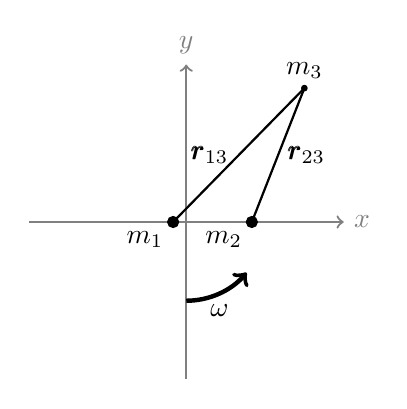
\begin{tikzpicture}

			\draw[gray, thick, ->] (-2, 0) -- (2, 0) node[anchor=west] {$x$};		% x-axis
			\draw[gray, thick, ->] (0, -2) -- (0, 2) node[anchor=south] {$y$};		% y-axis
			\filldraw[black] (-.167, 0) circle (2pt) node[anchor=north east] {$m_1$};
			\filldraw[black] (1-.167, 0) circle (2pt) node[anchor=north east] {$m_2$};
			\filldraw[black] (1.5, 1.7) circle(1pt) node[anchor=south] {$m_3$};
			\draw[black, thick] (-.167, 0) -- (1.5, 1.7) node[anchor=east, midway] {$\pmb{r}_{13}$}; 
			\draw[black, thick] (1-.167, 0) -- (1.5, 1.7) node[anchor=west, midway] {$\pmb{r}_{23}$};
			\draw[black, ->, ultra thick] (0, -1) arc (270:320:1) node[anchor=north, midway] {$\omega$};

		\end{tikzpicture}
		\label{f:coordinatesystem}
			\caption{Normalised co-ordinate system for the CR3BP -- $\omega$ and primary separation normalised to unity.}	
		\end{figure}
		%\begin{figure}
		%	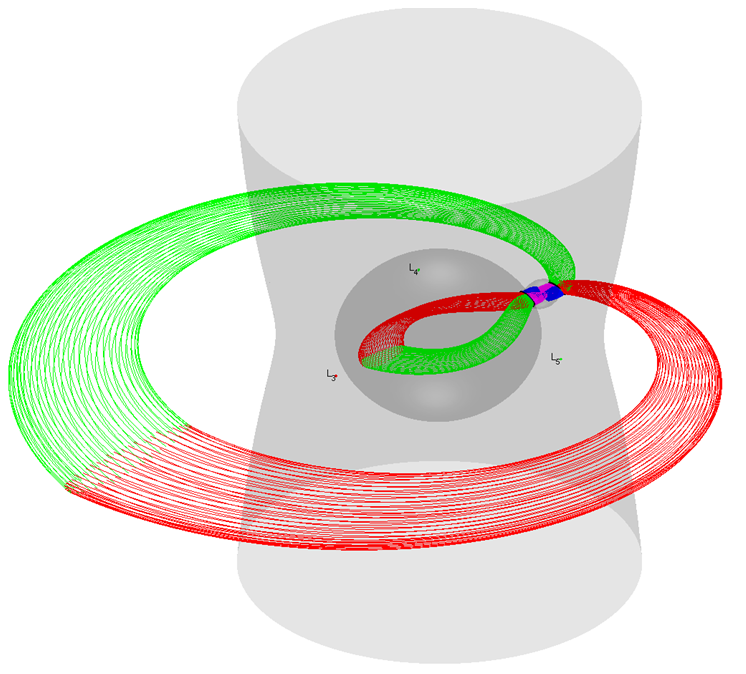
\includegraphics[width=\textwidth]{manifolds}
		%	\caption{\textit{Funky} dynamical behavour -- invariant manifold tubes}
		%\end{figure}
\end{frame}


%\begin{frame}[fragile]{Quirks of the CR3BP}
%	\begin{columns}
%		\column{.5\linewidth}
%			\begin{itemize}
%				\item Lagrangian points are points where the gravity of the two primaries `cancel out'
%				\item $L$-points (particularly Sun-Earth $L_1$) offer interesting characteristics for some science applications
%				\item Computing these (see right) \textit{periodic orbits} requires the use of numerical techniques, but is well understood
%			\end{itemize}
%		\column{0.5\ewidth}
%			\animategraphics[loop,width=\textwidth]{12}{gif/manifolds-}{0}{330}
%	\end{columns}
%
%\end{frame}
%\begin{frame}[fragile]{Introduction to Manifolds}
%	\small If we integrate orbits that exponentially approach and depart a certain periodic orbit in the CR3BP, we discover manifold tubes...
%	\begin{figure}
%		\centering
%		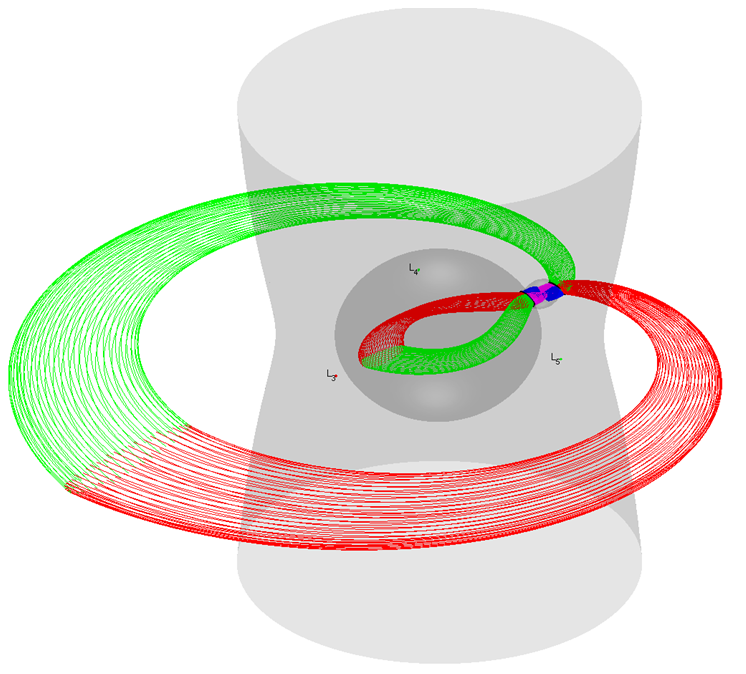
\includegraphics[height=.4\textheight]{manifolds}
%		\caption{\small Stable (green) and unstable (red) invariant manifolds associated to Earth-Moon L1. Source: Renkli Seyler, \url{https://renklisheyler.wordpress.com/research/motions-in-cr3bp/invariant-manifold-tubes/}}
%	\end{figure}
%	\small ...exploiting these dynamical phenomena can give rise to interesting applications
%
%\end{frame}
%
\begin{frame}[fragile]{Introduction to Manifolds}
	\small One dynamical phenomenon, manifold tubes -- orbits that approach and depart a periodic orbit in the CR3BP -- can be exploited to give new ways of transferring matter in phase space
	\begin{figure}
		\centering
		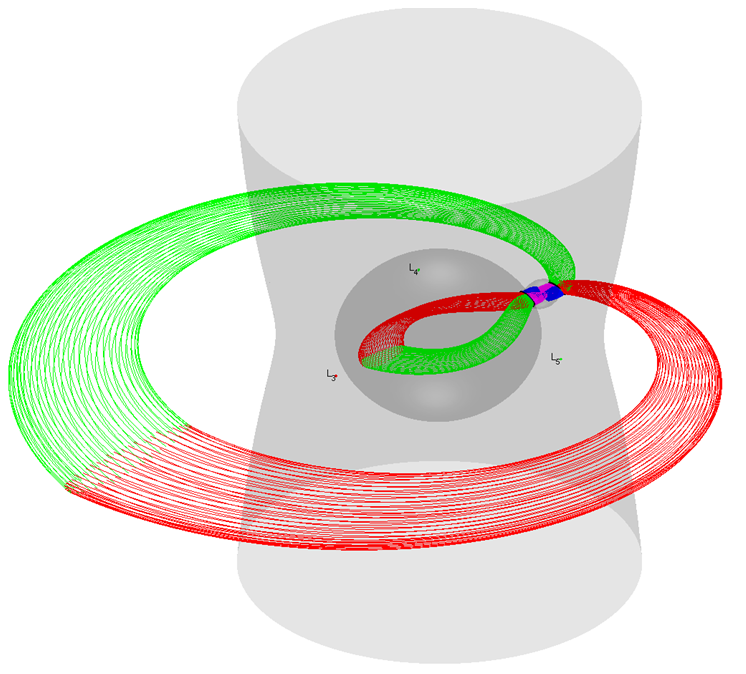
\includegraphics[height=.4\textheight]{manifolds}
		\caption{\small Stable (green) and unstable (red) invariant manifolds associated to Earth-Moon L1. Source: Renkli Seyler, \url{https://renklisheyler.wordpress.com/research/motions-in-cr3bp/invariant-manifold-tubes/}}
	\end{figure}
\end{frame}

\begin{frame}{Potential Applications}
	\begin{figure}
		\centering
		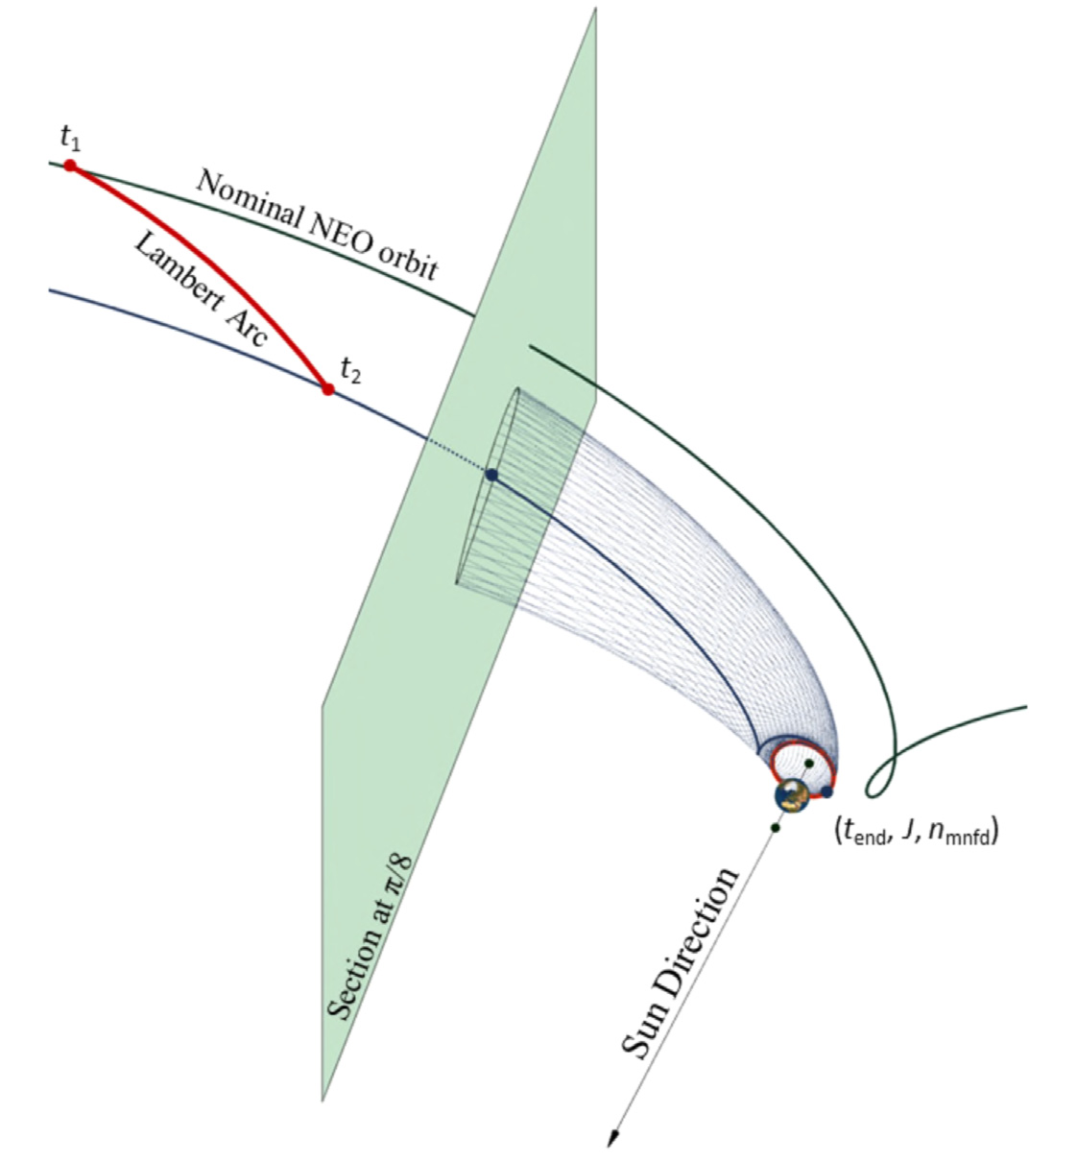
\includegraphics[height=.5\linewidth]{neo_retrieval.png}
		\caption{The use of stable invariant manifolds to perform an asteroid retrieval mission to Earth-Moon L2. \cite{Sanchez2016}}
	\end{figure}
\end{frame}

%\begin{frame}{Potential Applications - 2}
%	\begin{figure}
%		\centering
%		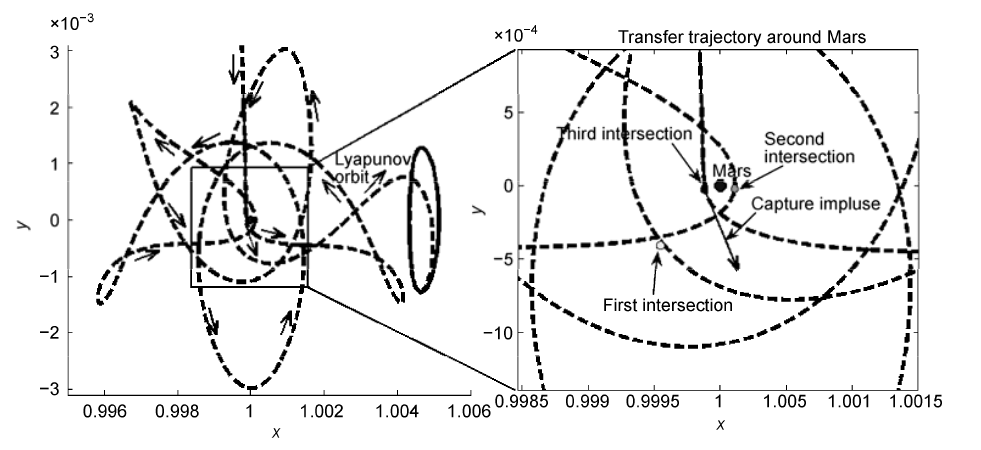
\includegraphics[height=.4\textheight]{interplanetary}
%		\caption{Earth Lagrangian point - Mars Lagrangian point interplanetary transfer via invariant manifolds and gravity assists. \cite{Shuai2013}}
%	\end{figure}
%\end{frame}

%\begin{frame}{Formal project proposal}
%	\small "The application of dynamical systems theory to space mission design has attracted attention for its' ability to construct new and unusual orbits that cannot be found through the classical approach to spacecraft trajectory design. In particular, the three-body problem yields many dynamical structures - stable and unstable manifolds and bounding surfaces - that provide phase-space structures for the transfer of objects into and from the smaller primary body. These dynamical structures can be exploited to construct `low-energy transfers', where the path of the third body exists as a harmony of gravitation, and can allow for the use of complex, non-Keplerian orbits to achieve mission objectives, as well as potential propellant savings.
%
%	Throughout this project, \emph{the underlying mathematics behind the three-body problem will be studied and appropriate analytical and numerical techniques will be implemented, which enable the systematic design of low-energy spacecraft trajectories by exploiting manifold dynamics around libration points}. A particular focus will be placed on the use of these dynamical phenomena to assemble spacecraft trajectories that exploit the characteristics of the Sun-Earth-Moon system."
%\end{frame}
%

\begin{frame}{Project aim and outcomes}
	\begin{itemize}
		\item The project will deliver a full case study for a mission in, and exploiting, the CR3BP
		\item To achieve this, the project sets the following aims:
			\begin{itemize}
				\item A comprehensive literature review on CR3BP theory, potential applications and numerical techniques for the contruction of orbits in the CR3BP
				\item A suitable mission selection that will exploit a range of features of the CR3BP
				\item A software bundle to allow for the computation of the mission analyses and orbit construction
			\end{itemize}
	\end{itemize}
\end{frame}

\begin{frame}{Project scope}
	\begin{itemize}
		\item The mathematics behind the CR3BP and its' dynamical phenomena
		\item The theory behind, and implementation of, numerical techniques for orbit construction including numerical integration, differential correction and optimisation
		\item Mission trade-offs and requirements
		\item Software analytics: code coverage, MC/DC coverage, static/dynamic program analysis and parallel processing techniques
	\end{itemize}
\end{frame}

%\begin{frame}{Project aim and outcomes}
%	\begin{itemize}
%		\item The project will aim to deliver a full case study for a mission in, and exploiting, the CR3BP
%		\item To achieve this, the project sets the following aims:
%			\begin{itemize}
%				\item A comprehensive literature review on CR3BP theory, potential applications and numerical techniques for the contruction of orbits in the CR3BP
%				\item A suitable mission selection that will exploit a range of features of the CR3BP
%				\item A software bundle to allow for the computation of the mission analyses and orbit construction
%			\end{itemize}
%	\end{itemize}
%\end{frame}
%
%\begin{frame}{Project scope}
%	\begin{itemize}
%		\item The mathematics behind the CR3BP and its' dynamical phenomena
%		\item The theory behind, and implementation of, numerical techniques for orbit construction including numerical integration, differential correction and optimisation
%		\item Mission trade-offs and requirements
%		\item Software analytics: code coverage, MC/DC coverage, static/dynamic program analysis and parallel processing techniques for minimising runtimes and ensuring program robustness
%	\end{itemize}
%\end{frame}
%	
%

\begin{frame}{(Very) provisional time plan}
	\centering
	\resizebox{\textwidth}{!}{
	\begin{ganttchart}{1}{24}
		  \gantttitle{IP provisional time plan}{24} \\
		  \gantttitlelist{1,...,24}{1} \\
		 % \ganttgroup{Group 1}{1}{7} \\
		  \ganttbar{Literature review \& mission selection}{1}{9} \\
		  %\ganttlinkedbar{Mission selection}{4}{4} \ganttnewline
		  \ganttlinkedmilestone{Check required knowledge}{10-12} \ganttnewline
		  \ganttlinkedbar{Programming software suite}{14}{18}\ganttnewline
		  \ganttlinkedbar{Finalising report write-up}{18}{24}\ganttnewline
		  %\ganttlinkedk{elem2}{elem3}
		  %\ganttlink{elem3}{elem4}
	\end{ganttchart}
}
\end{frame}

\begin{frame}{Any questions?}
	\begin{figure}
	\centering
		
%\begin{frame}[fragile]{Quirks of the CR3BP}
%	\animategraphics[autoplay, loop,height=.7\textheight, autoplay]{5}{gif/final_try-}{0}{265}
	\animategraphics[autoplay, loop,height=.5\textheight]{12}{gif/manifolds-}{0}{330}

	\caption{Single-shooting differential correction to construct a family of Lyapunov orbits around L$_1$; $\mu = 0.0121$}
	\end{figure}
\end{frame}

\begin{frame}{References}
	\bibliographystyle{apalike}
	\bibliography{demo.bib}
\end{frame}

\appendix

\begin{frame}{Supplementary slides -- zero velocity curves in the CR3BP}	\centering
	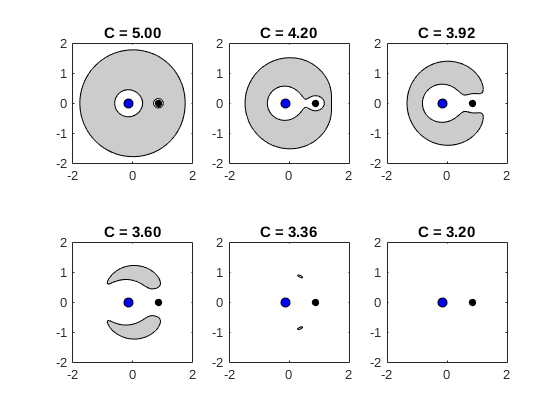
\includegraphics[width=.8\linewidth]{../figures/jacobiConstantEMSys}
\end{frame}

%\begin{frame}{Project aims, outcomes and scope}
%	\begin{itemize}
%		\item This project aims to lay out the underlying mathematics behind the existence and manipulation of manifold structures, and use numerical techniques to construct transfers involving them
%		\item The main project `deliverable' is a software suite that provides the computation of several case studies of these low-energy transfers
%		\item BUT the project was proposed to be open-ended, and gives a lot of wiggle room for taking a different path further down the line
%	\end{itemize}
%\end{frame}
%

%\begin{frame}{Project aim and outcomes}
%	\begin{itemize}
%		\item The project will aim to deliver a full case study for a mission in, and exploiting, the CR3BP
%		\item To achieve this, the project sets the following aims:
%			\begin{itemize}
%				\item A comprehensive literature review on CR3BP theory, potential applications and numerical techniques for the contruction of orbits in the CR3BP
%				\item A suitable mission selection that will exploit a range of features of the CR3BP
%				\item A software bundle to allow for the computation of the mission analyses and orbit construction
%			\end{itemize}
%	\end{itemize}
%\end{frame}
%
%\begin{frame}{Project scope}
%	\begin{itemize}
%		\item The mathematics behind the CR3BP and its' dynamical phenomena
%		\item The theory behind, and implementation of, numerical techniques for orbit construction including numerical integration, differential correction and optimisation
%		\item Mission trade-offs and requirements
%		\item Software analytics: code coverage, MC/DC coverage, static/dynamic program analysis and parallel processing techniques for minimising runtimes and ensuring program robustness
%	\end{itemize}
%\end{frame}
%			
%



%\begin{frame}{Provisional work plan}
%	\begin{itemize}
%		\item As mentioned, the project is proposed to be open-ended, and I won't know exactly which case studies I find most interesting until I''ve trie da fair few of them
%		\item As a result, the work plan sizes up to be:
%			\begin{itemize}
%				\item Between October 2017-May 2018:
%					\begin{itemize}
%						\item Do project.
%					\end{itemize}
%			\end{itemize}
%	\end{itemize}
%\end{frame}
%\section{Project Management Plan}
%
%\begin{frame}{Gantt Chart}
%	\themename supports 4 different titleformats:
%	\begin{itemize}
%		\item Regular
%		\item \textsc{Smallcaps}
%		\item \textsc{allsmallcaps}
%		\item ALLCAPS
%	\end{itemize}
%	They can either be set at once for every title type or individually.
%\end{frame}


%\begin{frame}{Training needs analysis}
%	\begin{itemize}
%		\item No faculty/facility-level training required
%	\end{itemize}
%\end{frame}

\begin{frame}{Current Project Progress}
	\begin{itemize}
		\item Self-proposal made it easy to do the literature review before Semester 1 started
		\item Mendeley library contains \textasciitilde 80 journal papers and books
		\item Already worked on (basic) underlying mathematics \& written this up into a reference document (16k words)
		\item Written code (MATLAB, Fortran03) to single-shoot some closed orbits
	\end{itemize}
\end{frame}



\end{document}
